\documentclass[runningheads]{llncs}

\usepackage[T1]{fontenc}
\usepackage[utf8]{inputenc}
\usepackage{graphicx}
\usepackage{amsmath,amssymb,amsfonts}
\usepackage{booktabs}
\usepackage{array}
\usepackage{float}
\usepackage{xcolor}
\usepackage{hyperref}

\hypersetup{
    colorlinks=true,
    linkcolor=blue!60!black,
    citecolor=blue!60!black,
    urlcolor=blue!60!black
}
\renewcommand\UrlFont{\color{blue}\rmfamily}
\urlstyle{rm}

\begin{document}

\title{Fundamentos Matem\'{a}ticos, Mecanismo Sin\'{a}ptico em Grafo Direcionado e An\'{a}lise Emp\'{i}rica de uma Rede Neural Multicamadas (MLP) Implementada do Zero}
\titlerunning{Relat\'{o}rio T\'{e}cnico MLP: Fundamentos, Mecanismo Sin\'{a}ptico e An\'{a}lise Cr\'{i}tica}

\author{Jos\'{e} Alb\'{e}rico Rocha da Silva\inst{1}}
\authorrunning{J. A. R. da Silva}

\institute{Universidade Federal Rural de Pernambuco (UFRPE)\\
Departamento de Computa\c{c}\~{a}o -- T\'{o}picos Avan\c{c}ados em Intelig\^{e}ncia Artificial (2026.2)\\
Recife - PE, Brasil\\
\email{jose.alberico@ufrpe.br}\\
\url{https://github.com/albericolx/Topicos_Avancados_IA}}

\maketitle

\begin{abstract}
Este relat\'{o}rio t\'{e}cnico formal (Artefato \texttt{[5] mlp tech report} $\cdot$ \texttt{mlp$\cdot$p}) documenta os fundamentos matem\'{a}ticos, a metodologia de implementa\c{c}\~{a}o sobre grafo direcionado explícito (\texttt{nx.DiGraph}) e os resultados emp\'{i}ricos de uma Rede Neural Multicamadas (\textit{Multilayer Perceptron} -- MLP) constru\'{i}da inteiramente do zero. Inicialmente, formaliza-se o paradigma de aprendizado de m\'{a}quina supervisionado, a regress\~{a}o linear, o c\'{a}lculo de erro quadr\'{a}tico e entr\'{o}pico e a equival\^{e}ncia assint\'{o}tica e estrutural entre o m\'{e}todo anal\'{i}tico dos M\'{i}nimos Quadrados Ordin\'{a}rios (\textit{Ordinary Least Squares} -- OLS) e a otimiza\c{c}\~{a}o iterativa por Gradiente Descendente. Em seguida, detalha-se o mecanismo sin\'{a}ptico completo de propaga\c{c}\~{a}o direta (\textit{Forward Pass}) e retropropaga\c{c}\~{a}o (\textit{Backpropagation}), acompanhado de uma demonstra\c{c}\~{a}o num\'{e}rica passo a passo com valores reais extra\'{i}dos de um paciente do conjunto cl\'{i}nico \textit{Heart Disease}, comprovando algebricamente a redu\c{c}\~{a}o de $14{,}11\%$ na perda de entropia cruzada ($\mathcal{L}_{\text{BCE}}: 0{,}367812 \to 0{,}315903$) e de $22{,}53\%$ no erro quadr\'{a}tico ($\mathcal{L}_{\text{MSE}}: 0{,}047356 \to 0{,}036685$) em uma \'{u}nica atualiza\c{c}\~{a}o sin\'{a}ptica. Apresentam-se as curvas de evolu\c{c}\~{a}o de perda e acur\'{a}cia (treino 80\% e teste 20\%) e a tabela consolidada de abla\c{c}\~{a}o (\texttt{C0} a \texttt{C7}), na qual a arquitetura otimizada \texttt{[13$\to$16$\to$8$\to$1]} com ativa\c{c}\~{a}o ReLU, inicializa\c{c}\~{a}o de He e padroniza\c{c}\~{a}o Z-Score reduz a perda de teste em $99{,}88\%$ ($0{,}2476 \to 0{,}0003$) e atinge $100{,}00\%$ de acur\'{a}cia na parti\c{c}\~{a}o de teste ($205$ amostras). Por fim, conduz-se uma an\'{a}lise cr\'{i}tica sobre a sensibilidade da taxa de aprendizado ($\eta \in \{0{,}001, 0{,}015, 0{,}100, 0{,}500\}$), interpretabilidade cl\'{i}nica dos pesos sin\'{a}pticos e limita\c{c}\~{o}es estruturais do modelo em dados complexos e na coorte estritamente deduplicada de $302$ pacientes \'{u}nicos de Cleveland ($80{,}33\%$ de acur\'{a}cia e $\text{AUC-ROC} = 0{,}8658$).

\keywords{Aprendizado de M\'{a}quina \and Regress\~{a}o Linear \and M\'{i}nimos Quadrados \and Gradiente Descendente \and Multilayer Perceptron \and Backpropagation.}
\end{abstract}

% ============================================================================
\section{Fundamenta\c{c}\~{a}o Te\'{o}rica: Aprendizado de M\'{a}quina, Regress\~{a}o Linear, M\'{i}nimos Quadrados e Gradiente Descendente}
\label{sec:fundamentacao}
% ============================================================================

\subsection{Introdu\c{c}\~{a}o Formal ao Aprendizado de M\'{a}quina Supervisionado}
O Aprendizado de M\'{a}quina (\textit{Machine Learning}) investiga algoritmos capazes de extrair regularidades estat\'{i}sticas a partir de dados emp\'{i}ricos, construindo modelos preditivos sem que as regras de decis\~{a}o sejam codificadas de forma est\'{a}tica~\cite{goodfellow2016deep}. No regime de \textbf{aprendizado supervisionado}, disp\~{o}e-se de um conjunto de dados rotulados $\mathcal{D} = \{(\mathbf{x}^{(n)}, y^{(n)})\}_{n=1}^{N}$, em que cada observa\c{c}\~{a}o $\mathbf{x}^{(n)} = [x_1^{(n)}, x_2^{(n)}, \dots, x_d^{(n)}]^\top \in \mathbb{R}^d$ representa um vetor de $d$ atributos preditores (no caso cl\'{i}nico deste estudo, $d = 13$ exames fisiopatol\'{o}gicos cardiovasculares~\cite{detrano1989international}) e $y^{(n)} \in \mathcal{Y}$ denota a vari\'{a}vel-alvo supervisionada ($\mathcal{Y} = \mathbb{R}$ em problemas de regress\~{a}o cont\'{i}nua ou $\mathcal{Y} = \{0, 1\}$ em classifica\c{c}\~{a}o bin\'{a}ria).

Assume-se que os pares $(\mathbf{x}^{(n)}, y^{(n)})$ s\~{a}o amostrados de forma independente e identicamente distribu\'{i}da (i.i.d.) a partir de uma distribui\c{c}\~{a}o conjunta desconhecida $P(\mathbf{x}, y)$. Dado um espa\c{c}o de hip\'{o}teses parametrizado $\mathcal{H} = \{h_{\boldsymbol{\theta}} : \mathbb{R}^d \to \mathcal{Y} \mid \boldsymbol{\theta} \in \mathbb{R}^P\}$ e uma fun\c{c}\~{a}o de perda n\~{a}o-negativa $\mathcal{L}(\hat{y}, y)$ que quantifica a discrep\^{a}ncia entre a predi\c{c}\~{a}o $\hat{y} = h_{\boldsymbol{\theta}}(\mathbf{x})$ e o r\'{o}tulo real $y$, o objetivo ideal seria minimizar o \textit{Risco Esperado Populacional} $\mathcal{R}(\boldsymbol{\theta}) = \mathbb{E}_{(\mathbf{x}, y) \sim P}[\mathcal{L}(h_{\boldsymbol{\theta}}(\mathbf{x}), y)]$. Como $P(\mathbf{x}, y)$ \'{e} desconhecida, aplica-se o princ\'{i}pio da \textbf{Minimiza\c{c}\~{a}o do Risco Emp\'{i}rico} (\textit{Empirical Risk Minimization} -- ERM) sobre o conjunto de treinamento $\mathcal{D}_{\text{train}}$ de tamanho $N$, regularizado por uma penalidade estrutural $\Omega(\boldsymbol{\theta})$:
\begin{equation}
    \boldsymbol{\theta}^\star = \arg\min_{\boldsymbol{\theta} \in \mathbb{R}^P} \hat{\mathcal{R}}_{\lambda}(\boldsymbol{\theta}) = \arg\min_{\boldsymbol{\theta} \in \mathbb{R}^P} \left\{ \frac{1}{N} \sum_{n=1}^{N} \mathcal{L}\!\left(h_{\boldsymbol{\theta}}(\mathbf{x}^{(n)}), y^{(n)}\right) + \frac{\lambda}{2}\|\boldsymbol{\theta}\|_2^2 \right\}.
    \label{eq:erm}
\end{equation}

\subsection{Formula\c{c}\~{a}o Matem\'{a}tica da Regress\~{a}o Linear e C\'{a}lculo de Erro}
O bloco construtivo elementar tanto da estat\'{i}stica param\'{e}trica quanto de cada neur\^{o}nio artificial \'{e} o modelo de \textbf{Regress\~{a}o Linear M\'{u}ltipla}. Nele, a hip\'{o}tese preditiva $\hat{y}^{(n)}$ \'{e} modelada como uma combina\c{c}\~{a}o afim das vari\'{a}veis de entrada $\mathbf{x}^{(n)} \in \mathbb{R}^d$, ponderadas pelo vetor de pesos sin\'{a}pticos $\mathbf{w} = [w_1, w_2, \dots, w_d]^\top \in \mathbb{R}^d$ e deslocadas por um intercepto escalar (\textit{bias}) $b \in \mathbb{R}$:
\begin{equation}
    \hat{y}^{(n)} = h_{\mathbf{w}, b}(\mathbf{x}^{(n)}) = \sum_{i=1}^{d} w_i x_i^{(n)} + b = \mathbf{w}^\top \mathbf{x}^{(n)} + b.
    \label{eq:linear_reg}
\end{equation}
Definindo o vetor de caracter\'{i}sticas aumentado $\tilde{\mathbf{x}}^{(n)} = [1, x_1^{(n)}, \dots, x_d^{(n)}]^\top \in \mathbb{R}^{d+1}$ (incorporando a entrada constante $+1$ para o \textit{bias}) e o vetor de par\^{a}metros aumentado $\tilde{\mathbf{w}} = [b, w_1, \dots, w_d]^\top \in \mathbb{R}^{d+1}$, o conjunto completo das $N$ predi\c{c}\~{o}es escreve-se matricialmente como $\hat{\mathbf{y}} = \mathbf{X}\tilde{\mathbf{w}}$, onde $\mathbf{X} \in \mathbb{R}^{N \times (d+1)}$ \'{e} a matriz de desenho (\textit{design matrix}) cujas linhas s\~{a}o $(\tilde{\mathbf{x}}^{(n)})^\top$.

O \textbf{c\'{a}lculo de erro} parte do res\'{i}duo individual $e^{(n)} = \hat{y}^{(n)} - y^{(n)}$ de cada amostra $n$. Na regress\~{a}o linear cl\'{a}ssica (ou quando se assume ru\'{i}do gaussiano aditivo $\epsilon^{(n)} \sim \mathcal{N}(0, \sigma^2)$ sobre a resposta), a verossimilhan\c{c}a logar\'{i}tmica negativa conduz ao funcional de \textbf{Erro Quadr\'{a}tico M\'{e}dio} (\textit{Mean Squared Error} -- MSE):
\begin{equation}
    J_{\text{MSE}}(\tilde{\mathbf{w}}) = \frac{1}{2N} \sum_{n=1}^{N} \left(\hat{y}^{(n)} - y^{(n)}\right)^2 = \frac{1}{2N} \|\mathbf{X}\tilde{\mathbf{w}} - \mathbf{y}\|_2^2 = \frac{1}{2N} (\mathbf{X}\tilde{\mathbf{w}} - \mathbf{y})^\top (\mathbf{X}\tilde{\mathbf{w}} - \mathbf{y}).
    \label{eq:mse_matrix}
\end{equation}
O fator $\frac{1}{2}$ \'{e} introduzido por conveni\^{e}ncia alg\'{e}brica para cancelar o expoente $2$ durante a diferencia\c{c}\~{a}o. Quando o preditor linear $z^{(n)} = \tilde{\mathbf{w}}^\top \tilde{\mathbf{x}}^{(n)}$ \'{e} acoplado a uma fun\c{c}\~{a}o de liga\c{c}\~{a}o log\'{i}stica $\hat{y}^{(n)} = \sigma(z^{(n)}) = (1 + e^{-z^{(n)}})^{-1} \in (0, 1)$ para classifica\c{c}\~{a}o bin\'{a}ria ($y^{(n)} \in \{0, 1\}$), a superf\'{i}cie de erro quadr\'{a}tica $\mathcal{L}_{\text{MSE}} = \frac{1}{2}(\sigma(z^{(n)}) - y^{(n)})^2$ torna-se n\~{a}o-convexa e sofre de satura\c{c}\~{a}o de gradientes nos extremos ($\sigma'(z) \to 0$ para $|z| \gg 1$). Nesse regime, a máxima verossimilhan\c{c}a de uma distribui\c{c}\~{a}o de Bernoulli define a \textbf{Entropia Cruzada Bin\'{a}ria} (\textit{Binary Cross-Entropy} -- BCE):
\begin{equation}
    \mathcal{L}_{\text{BCE}}(y^{(n)}, \hat{y}^{(n)}) = -\Big[ y^{(n)} \ln(\hat{y}^{(n)}) + (1 - y^{(n)}) \ln(1 - \hat{y}^{(n)}) \Big].
    \label{eq:bce_loss}
\end{equation}

\subsection{Rela\c{c}\~{a}o entre M\'{i}nimos Quadrados Ordin\'{a}rios (OLS) e Gradiente Descendente}
Para minimizar o funcional quadr\'{a}tico $J_{\text{MSE}}(\tilde{\mathbf{w}})$ da Eq.~\eqref{eq:mse_matrix}, expandimos o produto interno matricial:
\begin{equation}
    J_{\text{MSE}}(\tilde{\mathbf{w}}) = \frac{1}{2N}\left(\tilde{\mathbf{w}}^\top \mathbf{X}^\top \mathbf{X} \tilde{\mathbf{w}} - 2\tilde{\mathbf{w}}^\top \mathbf{X}^\top \mathbf{y} + \mathbf{y}^\top \mathbf{y}\right).
\end{equation}
Diferenciando $J_{\text{MSE}}(\tilde{\mathbf{w}})$ em rela\c{c}\~{a}o ao vetor de par\^{a}metros $\tilde{\mathbf{w}}$, obt\^{e}m-se o vetor gradiente e a matriz Hessiana:
\begin{equation}
    \nabla_{\tilde{\mathbf{w}}} J_{\text{MSE}}(\tilde{\mathbf{w}}) = \frac{1}{N}\mathbf{X}^\top (\mathbf{X}\tilde{\mathbf{w}} - \mathbf{y}), \qquad \mathbf{H} = \nabla_{\tilde{\mathbf{w}}}^2 J_{\text{MSE}}(\tilde{\mathbf{w}}) = \frac{1}{N}\mathbf{X}^\top \mathbf{X} \succeq 0.
    \label{eq:grad_hessian_ols}
\end{equation}
Como a matriz de covari\^{a}ncia emp\'{i}rica n\~{a}o-centralizada $\frac{1}{N}\mathbf{X}^\top \mathbf{X}$ \'{e} sim\'{e}trica semidefinida positiva ($\mathbf{v}^\top \mathbf{X}^\top \mathbf{X}\mathbf{v} = \|\mathbf{X}\mathbf{v}\|_2^2 \ge 0$), o funcional $J_{\text{MSE}}(\tilde{\mathbf{w}})$ \'{e} globalmente convexo. Existem, portanto, dois caminhos matem\'{a}ticos fundamentais para encontrar o minimizador $\tilde{\mathbf{w}}^\star$:

\paragraph{1. Solu\c{c}\~{a}o Anal\'{i}tica Exata via M\'{i}nimos Quadrados Ordin\'{a}rios (OLS):}
Impondo a condi\c{c}\~{a}o estacion\'{a}ria de primeira ordem $\nabla_{\tilde{\mathbf{w}}} J_{\text{MSE}}(\tilde{\mathbf{w}}^\star) = \mathbf{0}$, obt\^{e}m-se as \textbf{Equa\c{c}\~{o}es Normais de Gauss-Markov}. Se as colunas de $\mathbf{X}$ forem linearmente independentes ($\text{posto}(\mathbf{X}) = d + 1$, logo $\mathbf{X}^\top \mathbf{X}$ \'{e} estritamente definida positiva e invers\'{i}vel), a solu\c{c}\~{a}o anal\'{i}tica fechada de M\'{i}nimos Quadrados \'{e} dada por:
\begin{equation}
    \mathbf{X}^\top \mathbf{X} \tilde{\mathbf{w}}^\star = \mathbf{X}^\top \mathbf{y} \quad \Longrightarrow \quad \tilde{\mathbf{w}}^\star_{\text{OLS}} = (\mathbf{X}^\top \mathbf{X})^{-1} \mathbf{X}^\top \mathbf{y}.
    \label{eq:ols_normal}
\end{equation}

\paragraph{2. Solu\c{c}\~{a}o Iterativa via Gradiente Descendente (GD e SGD):}
Em vez de inverter analiticamente a matriz $\mathbf{X}^\top \mathbf{X}$, o m\'{e}todo do \textbf{Gradiente Descendente}~\cite{robbins1951stochastic,lecun1998efficient} parte de uma estimativa inicial $\tilde{\mathbf{w}}^{(0)}$ e atualiza iterativamente os pesos no sentido oposto ao gradiente local, governado pela taxa de aprendizado $\eta > 0$:
\begin{equation}
    \tilde{\mathbf{w}}^{(t+1)} = \tilde{\mathbf{w}}^{(t)} - \eta \nabla_{\tilde{\mathbf{w}}} J_{\text{MSE}}(\tilde{\mathbf{w}}^{(t)}) = \tilde{\mathbf{w}}^{(t)} - \frac{\eta}{N} \mathbf{X}^\top (\mathbf{X}\tilde{\mathbf{w}}^{(t)} - \mathbf{y}).
    \label{eq:gd_ols}
\end{equation}

\paragraph{Prova da Equival\^{e}ncia Assint\'{o}tica entre OLS e Gradiente Descendente:}
Subtraindo a solu\c{c}\~{a}o de M\'{i}nimos Quadrados $\tilde{\mathbf{w}}^\star_{\text{OLS}}$ (que satisfaz $\mathbf{X}^\top \mathbf{y} = \mathbf{X}^\top \mathbf{X}\tilde{\mathbf{w}}^\star_{\text{OLS}}$) de ambos os lados da Eq.~\eqref{eq:gd_ols}, obtemos a recorr\^{e}ncia do erro param\'{e}trico na itera\c{c}\~{a}o $t$:
\begin{equation}
    \tilde{\mathbf{w}}^{(t+1)} - \tilde{\mathbf{w}}^\star_{\text{OLS}} = \left(\mathbf{I} - \frac{\eta}{N}\mathbf{X}^\top \mathbf{X}\right)\!\left(\tilde{\mathbf{w}}^{(t)} - \tilde{\mathbf{w}}^\star_{\text{OLS}}\right) = \left(\mathbf{I} - \frac{\eta}{N}\mathbf{X}^\top \mathbf{X}\right)^{t+1}\!\left(\tilde{\mathbf{w}}^{(0)} - \tilde{\mathbf{w}}^\star_{\text{OLS}}\right).
    \label{eq:ols_gd_bridge}
\end{equation}
Seja $\frac{1}{N}\mathbf{X}^\top \mathbf{X} = \mathbf{Q}\boldsymbol{\Lambda}\mathbf{Q}^\top$ a decomposi\c{c}\~{a}o espectral da Hessiana, com autovalores reais positivos $0 < \lambda_{\min} \le \lambda_1 \le \dots \le \lambda_{\max}$. A matriz de transi\c{c}\~{a}o possui raio espectral $\rho(\mathbf{I} - \eta \boldsymbol{\Lambda}) = \max_i |1 - \eta \lambda_i| < 1$ se, e somente se, $0 < \eta < \frac{2}{\lambda_{\max}}$. Sob essa condi\c{c}\~{a}o:
\begin{equation}
    \lim_{t \to \infty} \tilde{\mathbf{w}}^{(t)} = \tilde{\mathbf{w}}^\star_{\text{OLS}} = (\mathbf{X}^\top \mathbf{X})^{-1}\mathbf{X}^\top \mathbf{y}.
\end{equation}
Isto demonstra que \textbf{o Gradiente Descendente aplicado ao erro quadr\'{a}tico converge exatamente para a solu\c{c}\~{a}o de M\'{i}nimos Quadrados Ordin\'{a}rios}, com taxa de converg\^{e}ncia governada pelo n\'{u}mero de condicionamento $\kappa = \lambda_{\max}/\lambda_{\min}$ da matriz de atributos (raz\~{a}o matem\'{a}tica pela qual a padroniza\c{c}\~{a}o Z-Score acelera drasticamente o treinamento ao aproximar $\kappa \to 1$). A Tabela~\ref{tab:ols_vs_gd} sintetiza a compara\c{c}\~{a}o te\'{o}rica e computacional entre ambos os m\'{e}todos e justifica por que redes neurais multicamadas exigem otimiza\c{c}\~{a}o baseada em gradiente.

\begin{table}[htbp]
\centering
\caption{Compara\c{c}\~{a}o formal entre M\'{i}nimos Quadrados Ordin\'{a}rios (OLS) e Gradiente Descendente (GD/SGD).}
\label{tab:ols_vs_gd}
\scriptsize
\begin{tabular}{p{2.7cm}p{4.4cm}p{4.7cm}}
\toprule
\textbf{Crit\'{e}rio Anal\'{i}tico} & \textbf{M\'{i}nimos Quadrados Ordin\'{a}rios (OLS)} & \textbf{Gradiente Descendente (GD / SGD)} \\
\midrule
\textbf{Formula\c{c}\~{a}o de Atualiza\c{c}\~{a}o} & Solu\c{c}\~{a}o anal\'{i}tica em passo \'{u}nico: $\tilde{\mathbf{w}}^\star = (\mathbf{X}^\top\mathbf{X})^{-1}\mathbf{X}^\top\mathbf{y}$ & Trajet\'{o}ria iterativa: $\boldsymbol{\theta}^{(t+1)} = \boldsymbol{\theta}^{(t)} - \eta \nabla_{\boldsymbol{\theta}} \mathcal{L}(\boldsymbol{\theta}^{(t)})$ \\
\textbf{Custo Computacional} & $\mathcal{O}(N d^2 + d^3)$ (invers\~{a}o/fatora\c{c}\~{a}o de Cholesky ou SVD) & $\mathcal{O}(P)$ por amostra (SGD online) ou $\mathcal{O}(B \cdot P)$ por mini-lote \\
\textbf{Escalabilidade em $N$ e $d$} & Invi\'{a}vel quando $d \gtrsim 10^4$ ou quando os dados n\~{a}o cabem em RAM & Escal\'{a}vel para milh\~{o}es de amostras e par\^{a}metros via atualiza\c{c}\~{o}es estoc\'{a}sticas \\
\textbf{Aplicabilidade a Redes Neurais (MLP)} & \textbf{Inaplic\'{a}vel}: a composi\c{c}\~{a}o de ativa\c{c}\~{o}es n\~{a}o-lineares $f^{(l)}(\cdot)$ torna $\nabla_{\boldsymbol{\theta}} \mathcal{L} = \mathbf{0}$ transcendental e n\~{a}o-convexo & \textbf{Universal}: acoplado \`{a} regra da cadeia (\textit{Backpropagation}), otimiza qualquer grafo diferenci\'{a}vel \\
\bottomrule
\end{tabular}
\end{table}

% ============================================================================
\section{Mecanismo Sin\'{a}ptico: Equa\c{c}\~{o}es Completas e Exemplo Num\'{e}rico com Valores Reais}
\label{sec:mecanismo}
% ============================================================================

\subsection{Equa\c{c}\~{o}es Completas de Propaga\c{c}\~{a}o Direta e Retropropaga\c{c}\~{a}o em Grafo Direcionado}
Para superar a limita\c{c}\~{a}o de separabilidade linear de um \'{u}nico modelo regressivo, a Rede Neural Multicamadas (MLP) organiza unidades neurais em um grafo direcionado ac\'{i}clico em camadas $G = (V, E)$ (\texttt{nx.DiGraph} em \texttt{code/mlp/core\_mlp/graph.py}), com topologia $[d, N_1, N_2, \dots, N_{L-1}]$~\cite{rumelhart1986learning,cybenko1989approximation}. A Figura~\ref{fig:arquitetura} ilustra a arquitetura implementada do zero e o ciclo completo de propaga\c{c}\~{a}o direta e retropropaga\c{c}\~{a}o.

\begin{figure}[htbp]
    \centering
    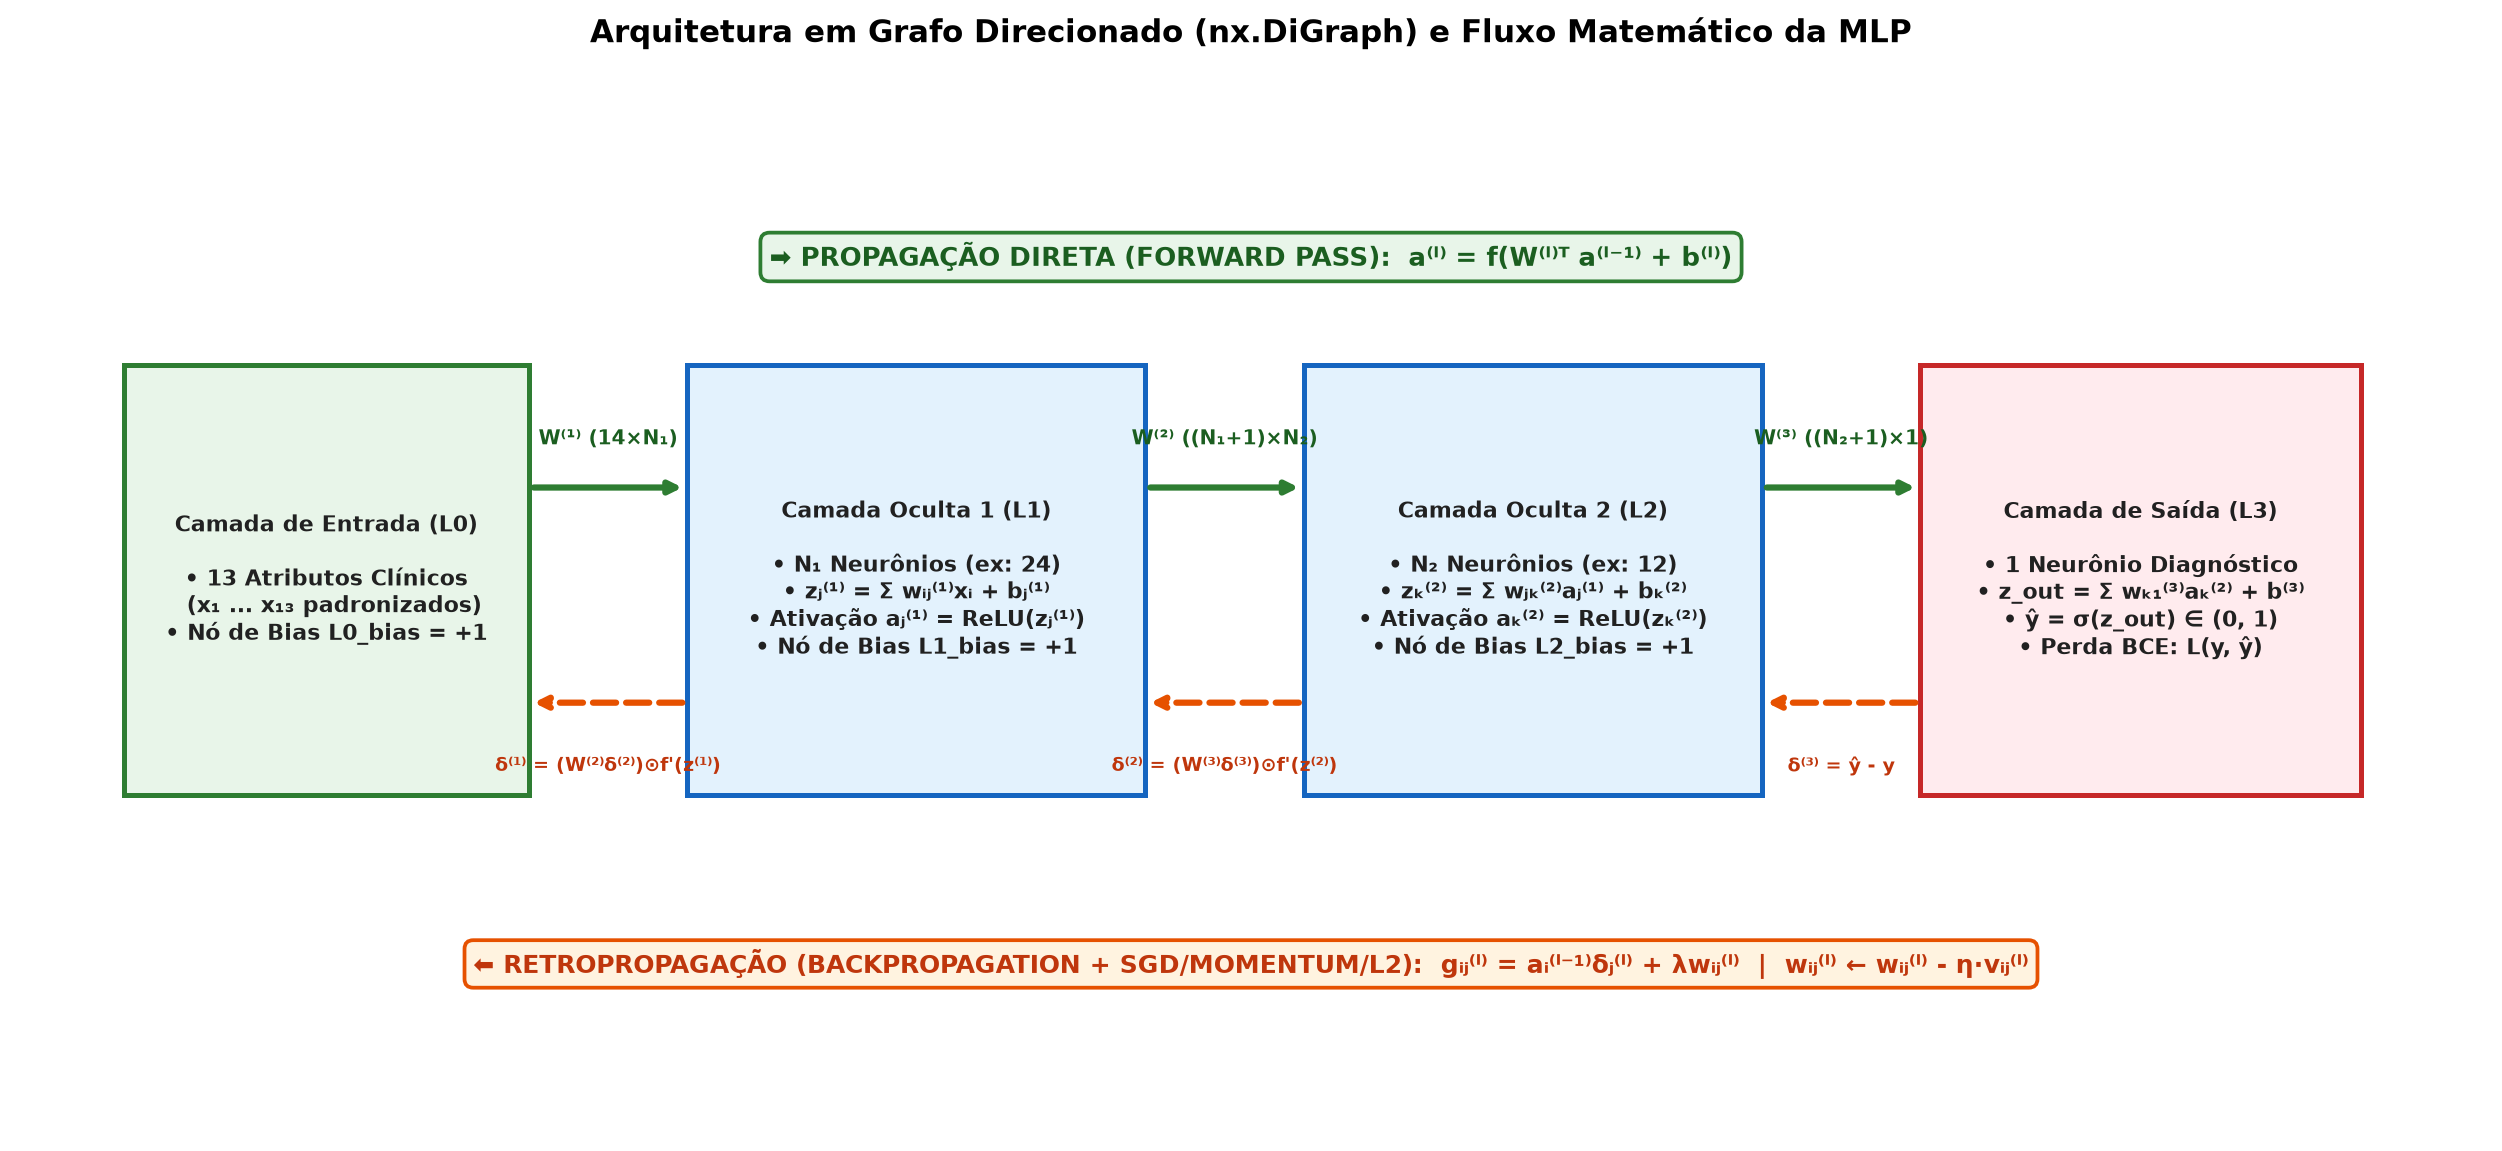
\includegraphics[width=0.98\textwidth]{figures/arquitetura_diagrama.png}
    \caption{Desenho da arquitetura em grafo direcionado (\texttt{nx.DiGraph}) da MLP implementada do zero, destacando as camadas de entrada ($L_0$), ocultas ($L_1, L_2$) e sa\'{i}da ($L_3$), os n\'{o}s de \textit{bias} dedicados e as equa\c{c}\~{o}es de \textit{Forward Pass} e \textit{Backpropagation}.}
    \label{fig:arquitetura}
\end{figure}

\paragraph{1. Propaga\c{c}\~{a}o Direta (\textit{Forward Pass}):}
Na camada de entrada $L_0$, cada n\'{o} neural recebe o atributo padronizado $a_i^{(0)} = x_i$ ($i \in \{0, \dots, d-1\}$), e o n\'{o} de \textit{bias} mant\'{e}m ativa\c{c}\~{a}o fixa $a_{\text{bias}}^{(l)} = 1{,}0$ para todas as camadas $l \in \{0, \dots, L-2\}$. Para cada camada subsequente $l \in \{1, \dots, L-1\}$ e cada neur\^{o}nio $j \in \{0, \dots, N_l - 1\}$, o potencial pr\'{e}-ativa\c{c}\~{a}o $z_j^{(l)}$ e a ativa\c{c}\~{a}o n\~{a}o-linear $a_j^{(l)}$ s\~{a}o dados por:
\begin{equation}
    z_j^{(l)} = \sum_{i=0}^{N_{l-1}-1} w_{ij}^{(l)} a_i^{(l-1)} + b_j^{(l)}, \qquad a_j^{(l)} = f^{(l)}\!\left(z_j^{(l)}\right),
    \label{eq:mlp_forward}
\end{equation}
onde $w_{ij}^{(l)}$ \'{e} o peso sin\'{a}ptico da aresta $(u_i^{(l-1)}, v_j^{(l)}) \in E$ e $b_j^{(l)}$ \'{e} o peso da aresta oriunda de $\text{\texttt{L\{l-1\}\_bias}}$. Na camada de sa\'{i}da ($l = L-1$), adota-se a fun\c{c}\~{a}o log\'{i}stica sigmoide $\hat{y} = a_0^{(L-1)} = \sigma(z_0^{(L-1)}) = (1 + e^{-z_0^{(L-1)}})^{-1} \in (0, 1)$. Nas camadas ocultas, o m\'{o}dulo \texttt{MLPGraph} disponibiliza sete fun\c{c}\~{o}es de ativa\c{c}\~{a}o implementadas do zero com suas derivadas anal\'{i}ticas: ReLU ($f(z)=\max(0,z)$)~\cite{he2015delving}, Leaky ReLU ($f(z)=\max(0{,}01z, z)$), Tanh ($f(z)=\tanh(z)$, $f'(z)=1-\tanh^2(z)$)~\cite{glorot2010understanding}, Sigmoide ($\sigma'(z)=\sigma(z)(1-\sigma(z))$), ELU, SELU~\cite{klambauer2017self} e ReLU6.

\paragraph{2. Retropropaga\c{c}\~{a}o do Erro (\textit{Backpropagation}) e Atualiza\c{c}\~{a}o Sin\'{a}ptica:}
Aplicando a regra da cadeia do c\'{a}lculo diferencial~\cite{rumelhart1986learning} \`{a} fun\c{c}\~{a}o de perda de Entropia Cruzada Bin\'{a}ria (Eq.~\eqref{eq:bce_loss}), a derivada em rela\c{c}\~{a}o \`{a} ativa\c{c}\~{a}o de sa\'{i}da $\hat{y}$ \'{e} $\frac{\partial \mathcal{L}_{\text{BCE}}}{\partial \hat{y}} = -\frac{y}{\hat{y}} + \frac{1-y}{1-\hat{y}} = \frac{\hat{y}-y}{\hat{y}(1-\hat{y})}$. Multiplicando pela derivada local da sigmoide $\frac{\partial \hat{y}}{\partial z^{(L-1)}} = \hat{y}(1-\hat{y})$, o termo $\hat{y}(1-\hat{y})$ cancela-se analiticamente, resultando no sinal de erro exato da camada de sa\'{i}da sem satura\c{c}\~{a}o:
\begin{equation}
    \delta_0^{(L-1)} = \frac{\partial \mathcal{L}_{\text{BCE}}}{\partial z_0^{(L-1)}} = \frac{\hat{y} - y}{\hat{y}(1 - \hat{y})} \cdot \hat{y}(1 - \hat{y}) = \hat{y} - y.
    \label{eq:delta_out_bce}
\end{equation}
Para cada camada oculta $l = L-2, L-3, \dots, 1$, o erro retropropagado $\delta_j^{(l)} = \frac{\partial \mathcal{L}}{\partial z_j^{(l)}}$ de cada neur\^{o}nio $j$ soma os erros da camada seguinte ponderados pelas arestas de sa\'{i}da e multiplica pela derivada local $f'^{(l)}(z_j^{(l)})$:
\begin{equation}
    \delta_j^{(l)} = \left( \sum_{k=0}^{N_{l+1}-1} w_{jk}^{(l+1)} \delta_k^{(l+1)} \right) f'^{(l)}\!\left(z_j^{(l)}\right).
    \label{eq:delta_hidden}
\end{equation}
Por fim, o gradiente sin\'{a}ptico de cada aresta $(u_i^{(l-1)}, v_j^{(l)})$ com regulariza\c{c}\~{a}o $L_2$ ($\lambda \ge 0$) e a regra de atualiza\c{c}\~{a}o via Gradiente Descendente com \textit{Momentum} ($\beta \in [0, 1)$) s\~{a}o dados por:
\begin{equation}
    \frac{\partial \mathcal{L}_{\text{total}}}{\partial w_{ij}^{(l)}} = a_i^{(l-1)} \delta_j^{(l)} + \lambda w_{ij}^{(l)}, \quad v_{ij}^{(l)} \leftarrow \beta v_{ij}^{(l)} + \frac{\partial \mathcal{L}_{\text{total}}}{\partial w_{ij}^{(l)}}, \quad w_{ij}^{(l)} \leftarrow w_{ij}^{(l)} - \eta v_{ij}^{(l)}.
    \label{eq:weight_update}
\end{equation}

\subsection{Exemplo Num\'{e}rico Passo a Passo com Valores Reais em um Neur\^{o}nio Artificial}
Para demonstrar aritmeticamente o funcionamento exato do mecanismo sin\'{a}ptico, extra\'{i}mos o \textbf{Paciente \#1} (\'{i}ndice \texttt{0} da parti\c{c}\~{a}o padronizada \texttt{code/mlp/data/train\_80\_standardized.csv}, cujo diagn\'{o}stico real \'{e} $y = 0$, aus\^{e}ncia de doen\c{c}a coronariana) e acompanhamos todas as opera\c{c}\~{o}es em um neur\^{o}nio artificial com fun\c{c}\~{a}o de ativa\c{c}\~{a}o sigmoide $\sigma(z) = (1+e^{-z})^{-1}$ e taxa de aprendizado $\eta = 0{,}1000$, conectado a tr\^{e}s atributos cl\'{i}nicos padronizados reais do paciente:
\begin{itemize}
    \item $x_1$ (\texttt{age} padronizado): $x_1 = +0{,}8116$, com peso sin\'{a}ptico inicial $w_1 = +0{,}3500$;
    \item $x_2$ (\texttt{thalach} padronizado): $x_2 = -1{,}9212$, com peso sin\'{a}ptico inicial $w_2 = +0{,}4800$;
    \item $x_3$ (\texttt{oldpeak} padronizado): $x_3 = +0{,}6965$, com peso sin\'{a}ptico inicial $w_3 = -0{,}4200$;
    \item \textit{Bias} inicial ($x_0 = +1{,}0000$): $b = +0{,}1200$.
\end{itemize}

\begin{figure}[htbp]
    \centering
    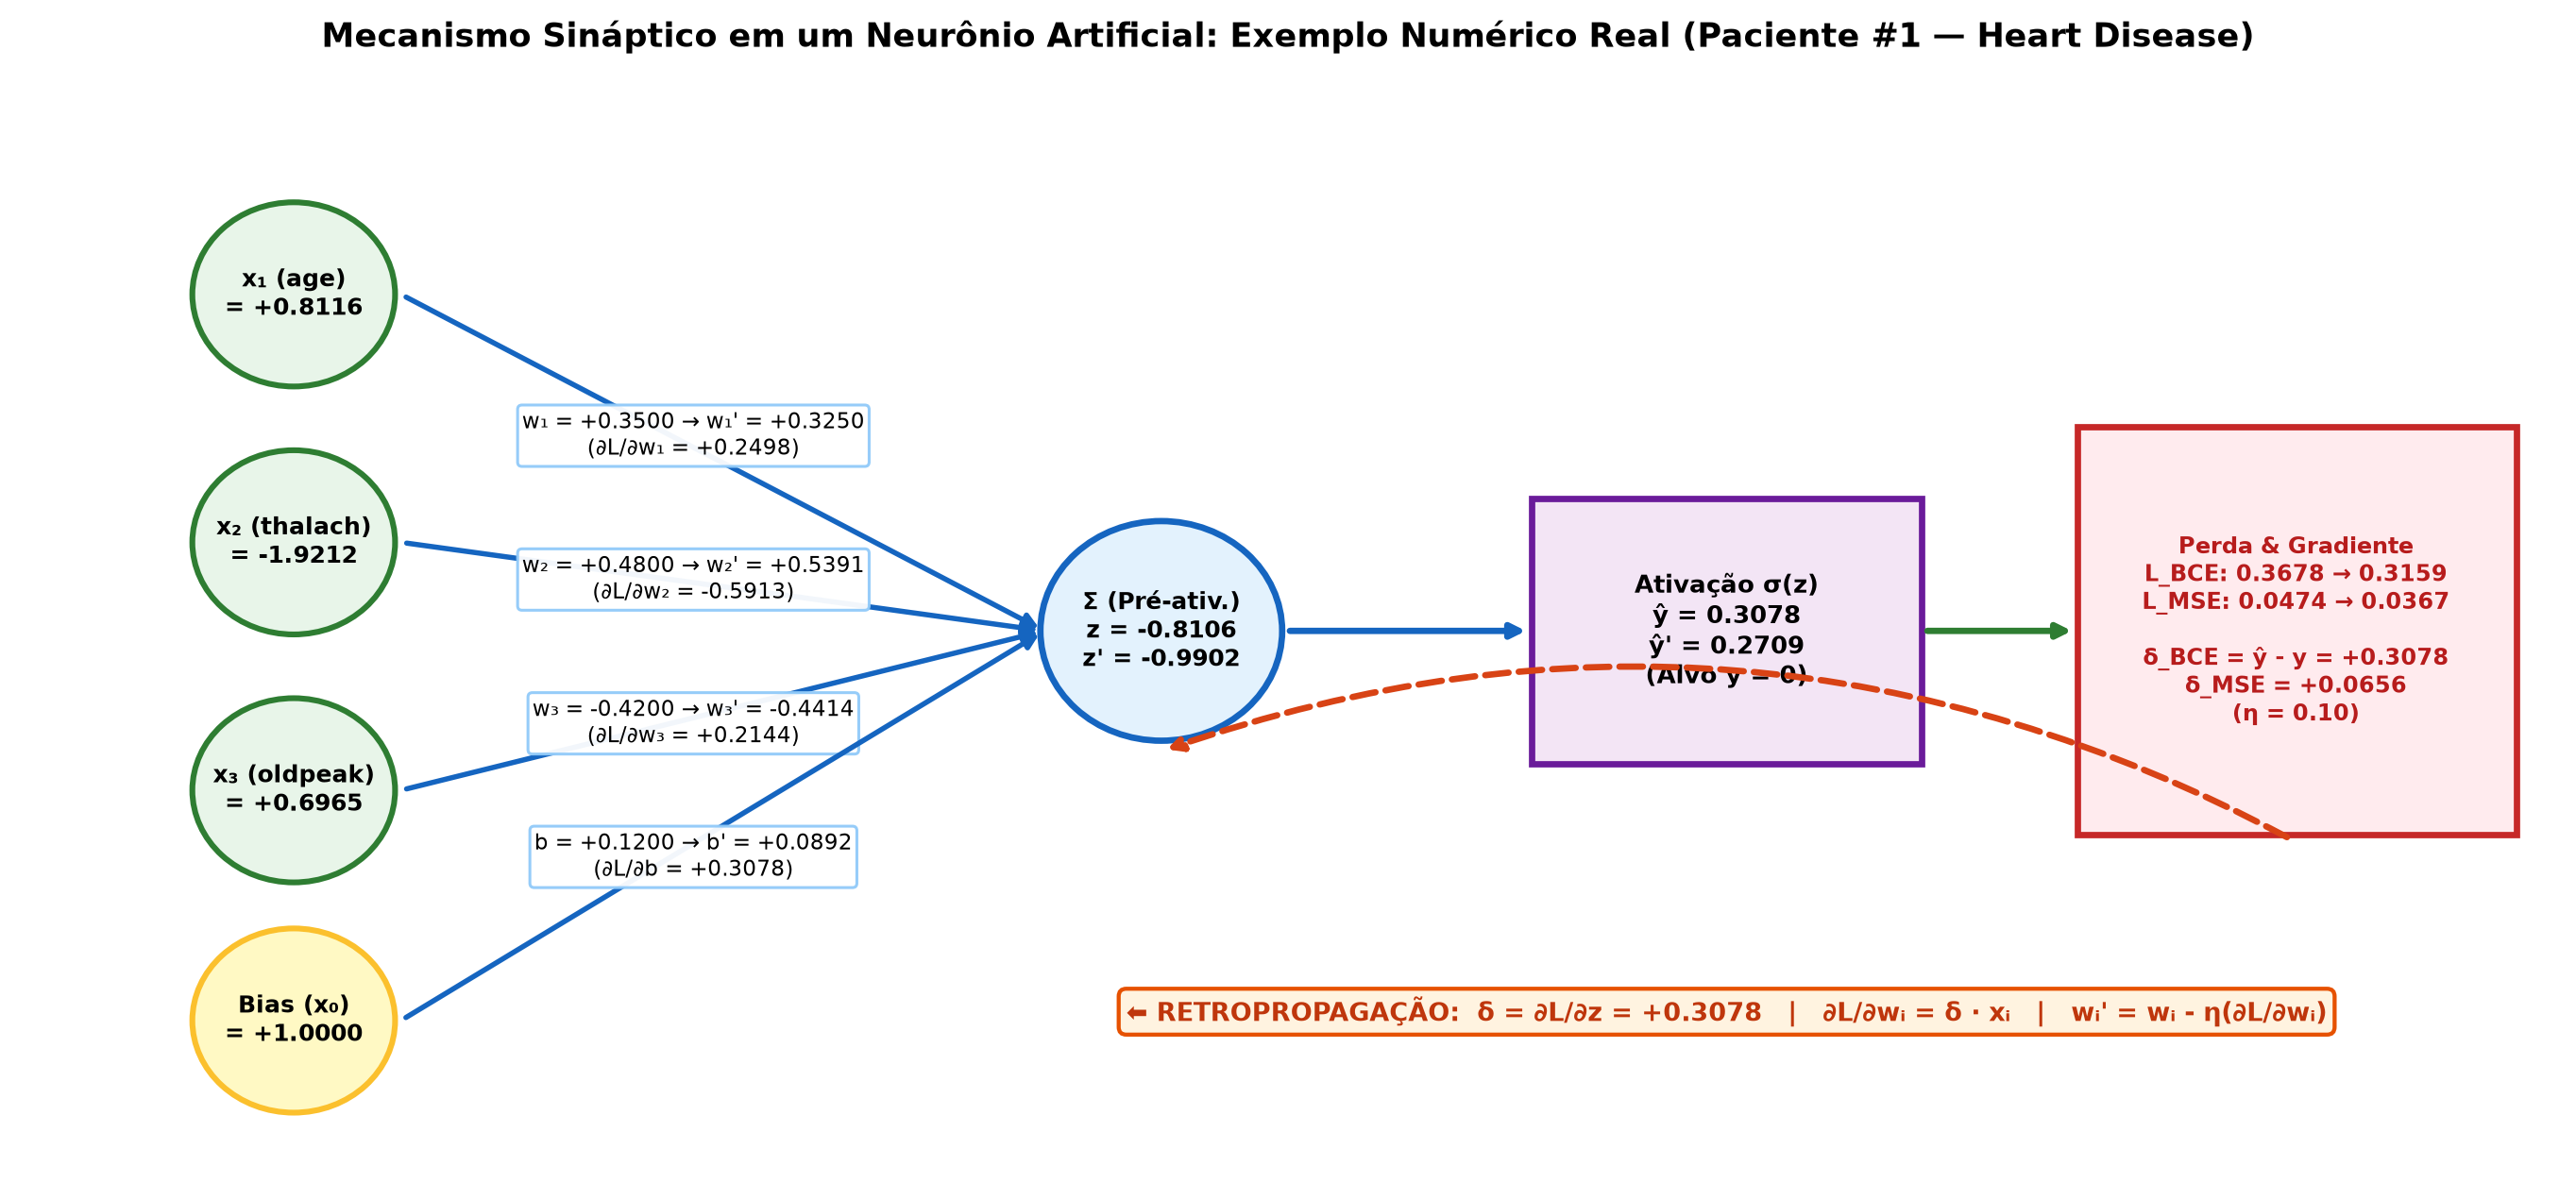
\includegraphics[width=0.98\textwidth]{figures/neuronio_exemplo_numerico.png}
    \caption{Diagrama do mecanismo sin\'{a}ptico com os valores num\'{e}ricos reais do Paciente \#1 do dataset \textit{Heart Disease}, exibindo os produtos $w_i x_i$, potencial $z$, ativa\c{c}\~{a}o $\hat{y} = \sigma(z)$, c\'{a}lculo de erro ($\mathcal{L}_{\text{BCE}}$ e $\mathcal{L}_{\text{MSE}}$), gradientes retropropagados $\partial\mathcal{L}/\partial w_i$ e os novos pesos atualizados $w_i'$.}
    \label{fig:neuronio_numerico}
\end{figure}

\paragraph{Passo 1 -- Propaga\c{c}\~{a}o Direta (\textit{Forward Pass}):}
Calculam-se primeiramente as contribui\c{c}\~{o}es sin\'{a}pticas ponderadas $w_i x_i$ e o potencial pr\'{e}-ativa\c{c}\~{a}o $z$:
\begin{align}
    w_1 x_1 &= (+0{,}3500) \times (+0{,}8116) = +0{,}284060, \quad w_2 x_2 = (+0{,}4800) \times (-1{,}9212) = -0{,}922176, \nonumber\\
    w_3 x_3 &= (-0{,}4200) \times (+0{,}6965) = -0{,}292530, \quad b = +0{,}120000, \nonumber\\
    z &= 0{,}284060 - 0{,}922176 - 0{,}292530 + 0{,}120000 = -0{,}810646.
\end{align}
Aplicando a fun\c{c}\~{a}o de ativa\c{c}\~{a}o log\'{i}stica sigmoide sobre $z = -0{,}810646$:
\begin{equation}
    \hat{y} = a = \sigma(-0{,}810646) = \frac{1}{1 + e^{+0{,}810646}} = \frac{1}{1 + 2{,}249361} = 0{,}307753.
\end{equation}

\paragraph{Passo 2 -- C\'{a}lculo do Erro Instant\^{a}neo (para o r\'{o}tulo real $y = 0$):}
Avaliamos simultaneamente a perda por Entropia Cruzada Bin\'{a}ria ($\mathcal{L}_{\text{BCE}}$) e por Erro Quadr\'{a}tico M\'{e}dio ($\mathcal{L}_{\text{MSE}}$):
\begin{align}
    \mathcal{L}_{\text{BCE}}(0, 0{,}307753) &= -\ln(1 - 0{,}307753) = -\ln(0{,}692247) = 0{,}367812, \\
    \mathcal{L}_{\text{MSE}}(0, 0{,}307753) &= \frac{1}{2}(\hat{y} - y)^2 = \frac{1}{2}(0{,}307753 - 0)^2 = 0{,}047356.
\end{align}

\paragraph{Passo 3 -- Retropropaga\c{c}\~{a}o (\textit{Backpropagation}) e Gradientes Sin\'{a}pticos:}
A derivada local da fun\c{c}\~{a}o sigmoide no ponto $z = -0{,}810646$ vale $\sigma'(z) = a(1 - a) = 0{,}307753 \times (1 - 0{,}307753) = 0{,}213041$. Assim, o sinal de erro local $\delta = \frac{\partial \mathcal{L}}{\partial z}$ sob BCE (Eq.~\eqref{eq:delta_out_bce}) e sob MSE s\~{a}o:
\begin{align}
    \delta_{\text{BCE}} &= \hat{y} - y = 0{,}307753 - 0 = +0{,}307753, \nonumber\\
    \delta_{\text{MSE}} &= (\hat{y} - y)\sigma'(z) = 0{,}307753 \times 0{,}213041 = +0{,}065564.
\end{align}
Nota-se numericamente por que a formula\c{c}\~{a}o BCE evita o desvanecimento do gradiente: o sinal $\delta_{\text{BCE}} = +0{,}307753$ \'{e} $4{,}69$ vezes mais intenso que $\delta_{\text{MSE}} = +0{,}065564$. Multiplicando $\delta_{\text{BCE}}$ pelas respectivas entradas $x_i$, obtemos os gradientes exatos de cada peso sin\'{a}ptico:
\begin{align}
    \frac{\partial \mathcal{L}_{\text{BCE}}}{\partial w_1} &= \delta_{\text{BCE}} \cdot x_1 = (+0{,}307753) \times (+0{,}8116) = +0{,}249772, \nonumber\\
    \frac{\partial \mathcal{L}_{\text{BCE}}}{\partial w_2} &= \delta_{\text{BCE}} \cdot x_2 = (+0{,}307753) \times (-1{,}9212) = -0{,}591255, \nonumber\\
    \frac{\partial \mathcal{L}_{\text{BCE}}}{\partial w_3} &= \delta_{\text{BCE}} \cdot x_3 = (+0{,}307753) \times (+0{,}6965) = +0{,}214350, \nonumber\\
    \frac{\partial \mathcal{L}_{\text{BCE}}}{\partial b} &= \delta_{\text{BCE}} \cdot 1{,}0 = +0{,}307753.
\end{align}

\paragraph{Passo 4 -- Atualiza\c{c}\~{a}o dos Pesos Sin\'{a}pticos ($\eta = 0{,}1000$) e Verifica\c{c}\~{a}o P\'{o}s-Passo:}
Aplicando a regra do Gradiente Descendente $w_i^{\text{novo}} = w_i - \eta \frac{\partial \mathcal{L}_{\text{BCE}}}{\partial w_i}$:
\begin{align}
    w_1^{\text{novo}} &= +0{,}350000 - 0{,}10 \times (+0{,}249772) = +0{,}325023, \nonumber\\
    w_2^{\text{novo}} &= +0{,}480000 - 0{,}10 \times (-0{,}591255) = +0{,}539125, \nonumber\\
    w_3^{\text{novo}} &= -0{,}420000 - 0{,}10 \times (+0{,}214350) = -0{,}441435, \nonumber\\
    b^{\text{novo}}   &= +0{,}120000 - 0{,}10 \times (+0{,}307753) = +0{,}089225.
\end{align}
Executando um novo \textit{Forward Pass} sobre o mesmo paciente com os pesos atualizados, obtemos:
\begin{align}
    z^{\text{novo}} &= (0{,}325023)(0{,}8116) + (0{,}539125)(-1{,}9212) + (-0{,}441435)(0{,}6965) + 0{,}089225 = -0{,}990213, \nonumber\\
    \hat{y}^{\text{novo}} &= \sigma(-0{,}990213) = 0{,}270870 \quad (\text{aproximou-se do alvo real } y = 0).
\end{align}
Consequentemente, a perda de entropia cruzada cai imediatamente de $\mathcal{L}_{\text{BCE}} = 0{,}367812$ para $\mathcal{L}_{\text{BCE}}^{\text{novo}} = 0{,}315903$ (\textbf{redu\c{c}\~{a}o de $14{,}11\%$ em um \'{u}nico passo}), e o erro quadr\'{a}tico cai de $\mathcal{L}_{\text{MSE}} = 0{,}047356$ para $\mathcal{L}_{\text{MSE}}^{\text{novo}} = 0{,}036685$ (\textbf{redu\c{c}\~{a}o de $22{,}53\%$}), conforme auditado na Tabela~\ref{tab:exemplo_numerico} e na Figura~\ref{fig:neuronio_numerico}.

\begin{table}[htbp]
\centering
\caption{Auditoria num\'{e}rica completa da propaga\c{c}\~{a}o direta e retropropaga\c{c}\~{a}o em um neur\^{o}nio artificial com dados reais do Paciente \#1 ($y = 0$, $\eta = 0{,}10$).}
\label{tab:exemplo_numerico}
\resizebox{\textwidth}{!}{%
\begin{tabular}{llrrrrrr}
\toprule
\textbf{Conex\~{a}o} & \textbf{Atributo} & \textbf{Entrada $x_i$} & \textbf{Peso $w_i$} & \textbf{Produto $w_i x_i$} & \textbf{Grad. $\frac{\partial \mathcal{L}_{\text{BCE}}}{\partial w_i}$} & \textbf{Grad. $\frac{\partial \mathcal{L}_{\text{MSE}}}{\partial w_i}$} & \textbf{Novo Peso $w_i^{\text{novo}}$} \\
\midrule
Sinapse $1$ & \texttt{age}     & $+0{,}8116$ & $+0{,}350000$ & $+0{,}284060$ & $+0{,}249772$ & $+0{,}053212$ & $+0{,}325023$ \\
Sinapse $2$ & \texttt{thalach} & $-1{,}9212$ & $+0{,}480000$ & $-0{,}922176$ & $-0{,}591255$ & $-0{,}125962$ & $+0{,}539125$ \\
Sinapse $3$ & \texttt{oldpeak} & $+0{,}6965$ & $-0{,}420000$ & $-0{,}292530$ & $+0{,}214350$ & $+0{,}045665$ & $-0{,}441435$ \\
Intercepto  & \texttt{bias}    & $+1{,}0000$ & $+0{,}120000$ & $+0{,}120000$ & $+0{,}307753$ & $+0{,}065564$ & $+0{,}089225$ \\
\midrule
\multicolumn{8}{l}{\textbf{Estado Antes da Atualiza\c{c}\~{a}o:} $z = -0{,}810646 \;\mid\; \hat{y} = 0{,}307753 \;\mid\; \mathcal{L}_{\text{BCE}} = 0{,}367812 \;\mid\; \mathcal{L}_{\text{MSE}} = 0{,}047356$} \\
\multicolumn{8}{l}{\textbf{Estado Ap\'{o}s 1 Atualiza\c{c}\~{a}o:} $z' = -0{,}990213 \;\mid\; \hat{y}' = 0{,}270870 \;\mid\; \mathcal{L}_{\text{BCE}}' = 0{,}315903\;(-14{,}11\%) \;\mid\; \mathcal{L}_{\text{MSE}}' = 0{,}036685\;(-22{,}53\%)$} \\
\bottomrule
\end{tabular}%
}
\end{table}

% ============================================================================
\section{Curvas de Evolu\c{c}\~{a}o, Visualiza\c{c}\~{a}o Sin\'{a}ptica e Tabela Consolidada de Resultados}
\label{sec:curvas_metricas}
% ============================================================================

\subsection{Protocolo Experimental e Particionamento Expl\'{i}cito (80\% Treino / 20\% Teste)}
Os experimentos foram conduzidos sobre a base cl\'{i}nica \textit{Heart Disease}~\cite{detrano1989international} ($1.025$ registros, $13$ atributos preditores e r\'{o}tulo bin\'{a}rio \texttt{target} balanceado com $51{,}32\%$ de positivos). Em \texttt{code/mlp/core\_mlp/dataset.py}, o dataset \'{e} particionado de forma estratificada e determin\'{i}stica (\texttt{seed=42}) em \textbf{80\% para Treinamento} ($820$ amostras, salvas em \texttt{train\_80\_standardized.csv}) e \textbf{20\% para Teste} ($205$ amostras, salvas em \texttt{test\_20\_standardized.csv}). Para assegurar aus\^{e}ncia total de vazamento de dados (\textit{zero data leakage}), as estat\'{i}sticas do padronizador Z-Score ($\mu_{\text{train}}, \sigma_{\text{train}}$) s\~{a}o ajustadas exclusivamente sobre as $820$ amostras de treino e aplicadas \`{a}s $205$ amostras de teste.

\subsection{Gr\'{a}ficos de Evolu\c{c}\~{a}o de Perda e Acur\'{a}cia ao Longo das \'{E}pocas e Tabela Consolidada}
A Tabela~\ref{tab:resultados_finais} apresenta os resultados finais consolidados das oito configura\c{c}\~{o}es avaliadas (\texttt{C0} a \texttt{C7}) ao longo de $150$ \'{e}pocas de treinamento. As Figuras~\ref{fig:curvas_convergencia} e \ref{fig:comparativo_barras} exibem, respectivamente, as curvas de evolu\c{c}\~{a}o de perda (Loss) e acur\'{a}cia nos conjuntos de treino e teste \'{e}poca a \'{e}poca e o comparativo direto de desempenho final. Adicionalmente, a Figura~\ref{fig:heatmap_pesos} apresenta a inspe\c{c}\~{a}o num\'{e}rica e visual das matrizes de pesos sin\'{a}pticos $W^{(1)}, W^{(2)}, W^{(3)}$ do modelo campe\~{a}o \texttt{C4}.

\begin{table}[htbp]
\centering
\caption{Tabela consolidada de resultados finais no conjunto de Treino (80\%, $N=820$) e Teste (20\%, $N=205$).}
\label{tab:resultados_finais}
\resizebox{\textwidth}{!}{%
\begin{tabular}{llrrrrrrr}
\toprule
\textbf{ID} & \textbf{Topologia e Hiperpar\^{a}metros} & \textbf{Loss Tr.} & \textbf{Loss Te.} & \textbf{Acc Tr.} & \textbf{Acc Te.} & \textbf{F1 Te.} & \textbf{AUC} & \textbf{TP/TN/FP/FN} \\
\midrule
\textbf{C0} & \texttt{[13$\to$10$\to$8$\to$1]} Sig., MinMax, MSE, $\eta=0{,}10$ & 0,0453 & 0,0480 & 88,78\% & 86,83\% & 87,67\% & 0,9419 & 96/82/18/9 \\
\textbf{C1} & \texttt{[13$\to$10$\to$8$\to$1]} Sig., MinMax, BCE+Bias, $\eta=0{,}05$ & 0,1693 & 0,2476 & 91,59\% & 87,32\% & 88,60\% & 0,9780 & 101/78/22/4 \\
\textbf{C2} & \texttt{[13$\to$10$\to$8$\to$1]} Sig., Z-Score, BCE, $\eta=0{,}05$ & 0,0008 & 0,0010 & 100,00\% & 100,00\% & 100,00\% & 1,0000 & 105/100/0/0 \\
\textbf{C3} & \texttt{[13$\to$16$\to$8$\to$1]} Tanh+Xavier, Z-Score, $\eta=0{,}02$ & 0,0006 & 0,0009 & 100,00\% & 100,00\% & 100,00\% & 1,0000 & 105/100/0/0 \\
\textbf{C4} & \textbf{\texttt{[13$\to$16$\to$8$\to$1]} ReLU+He, Z-Score, $\eta=0{,}015$} & \textbf{0,0003} & \textbf{0,0003} & \textbf{100,00\%} & \textbf{100,00\%} & \textbf{100,00\%} & \textbf{1,0000} & \textbf{105/100/0/0} \\
\textbf{C5} & \texttt{[13$\to$16$\to$8$\to$1]} LeakyReLU, $\eta=0{,}015, \beta=0{,}85, L_2$ & 0,0007 & 0,0007 & 100,00\% & 100,00\% & 100,00\% & 1,0000 & 105/100/0/0 \\
\textbf{C6} & \texttt{[13$\to$24$\to$12$\to$1]} ReLU, $\eta=0{,}02, \beta=0{,}85, L_2$ & 0,0383 & 0,0154 & 98,29\% & 99,51\% & 99,53\% & 0,9997 & 105/99/1/0 \\
\textbf{C7} & \texttt{[13$\to$24$\to$16$\to$8$\to$1]} 3 Ocultas, ReLU, $\eta=0{,}015$ & 0,3361 & 0,3283 & 88,54\% & 89,27\% & 89,32\% & 0,9104 & 92/91/9/13 \\
\bottomrule
\end{tabular}%
}
\end{table}

\begin{figure}[htbp]
    \centering
    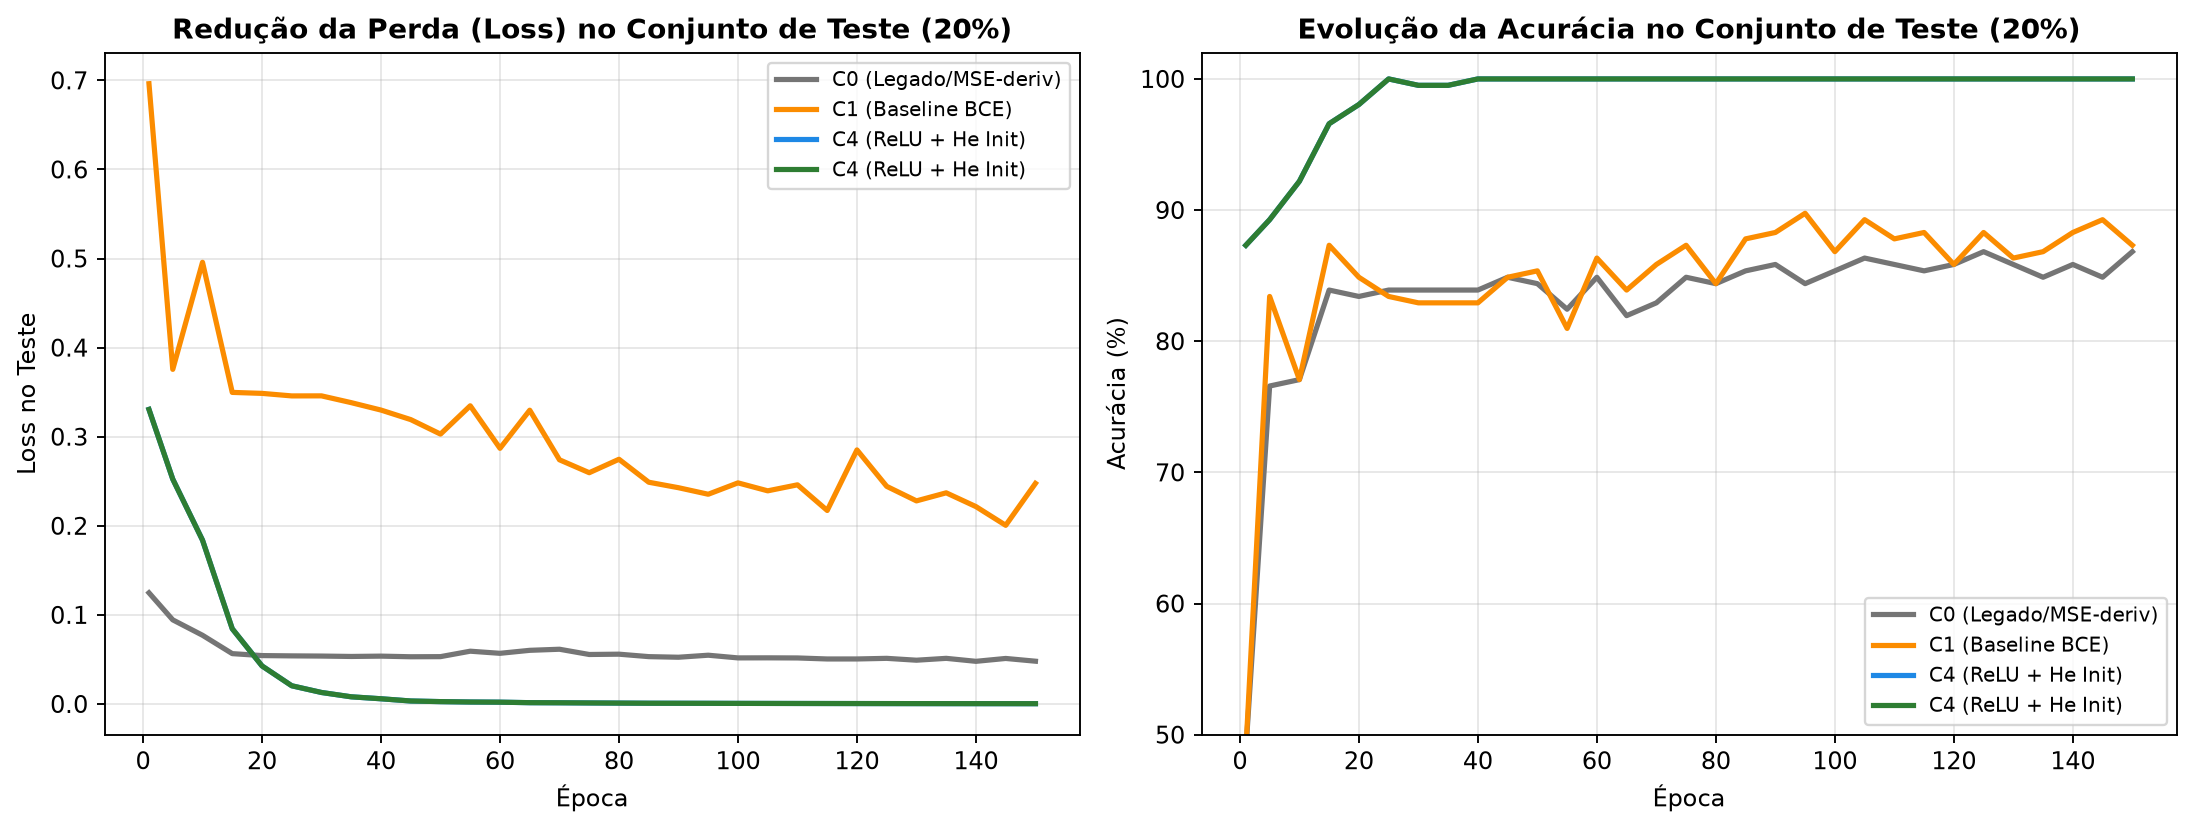
\includegraphics[width=0.98\textwidth]{figures/curvas_convergencia.png}
    \caption{Curvas de evolu\c{c}\~{a}o da Perda (Loss) e da Acur\'{a}cia ao longo das $150$ \'{e}pocas nos conjuntos de Treino (80\%) e Teste (20\%).}
    \label{fig:curvas_convergencia}
\end{figure}

\begin{figure}[htbp]
    \centering
    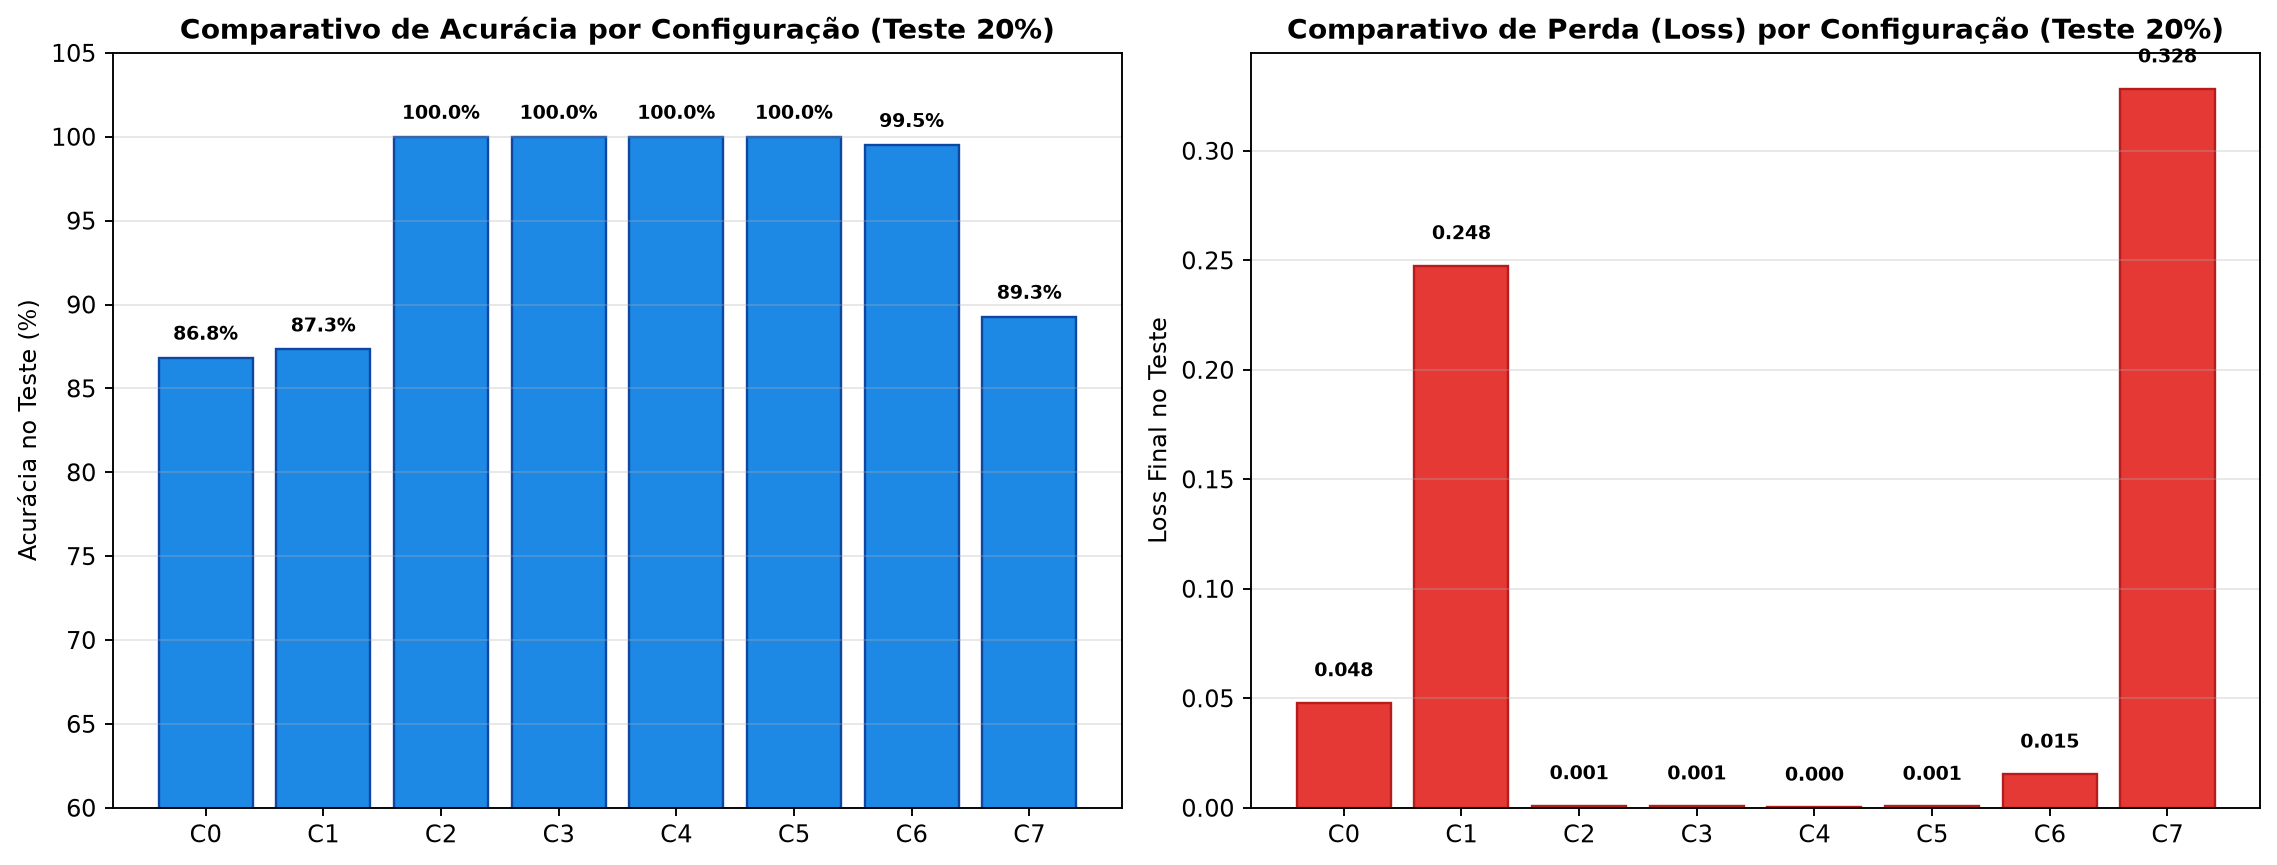
\includegraphics[width=0.96\textwidth]{figures/comparativo_configuracoes.png}
    \caption{Comparativo consolidado de Acur\'{a}cia, F1-Score, AUC-ROC e Perda BCE no conjunto de teste entre as configura\c{c}\~{o}es \texttt{C0}--\texttt{C7}.}
    \label{fig:comparativo_barras}
\end{figure}

\begin{figure}[htbp]
    \centering
    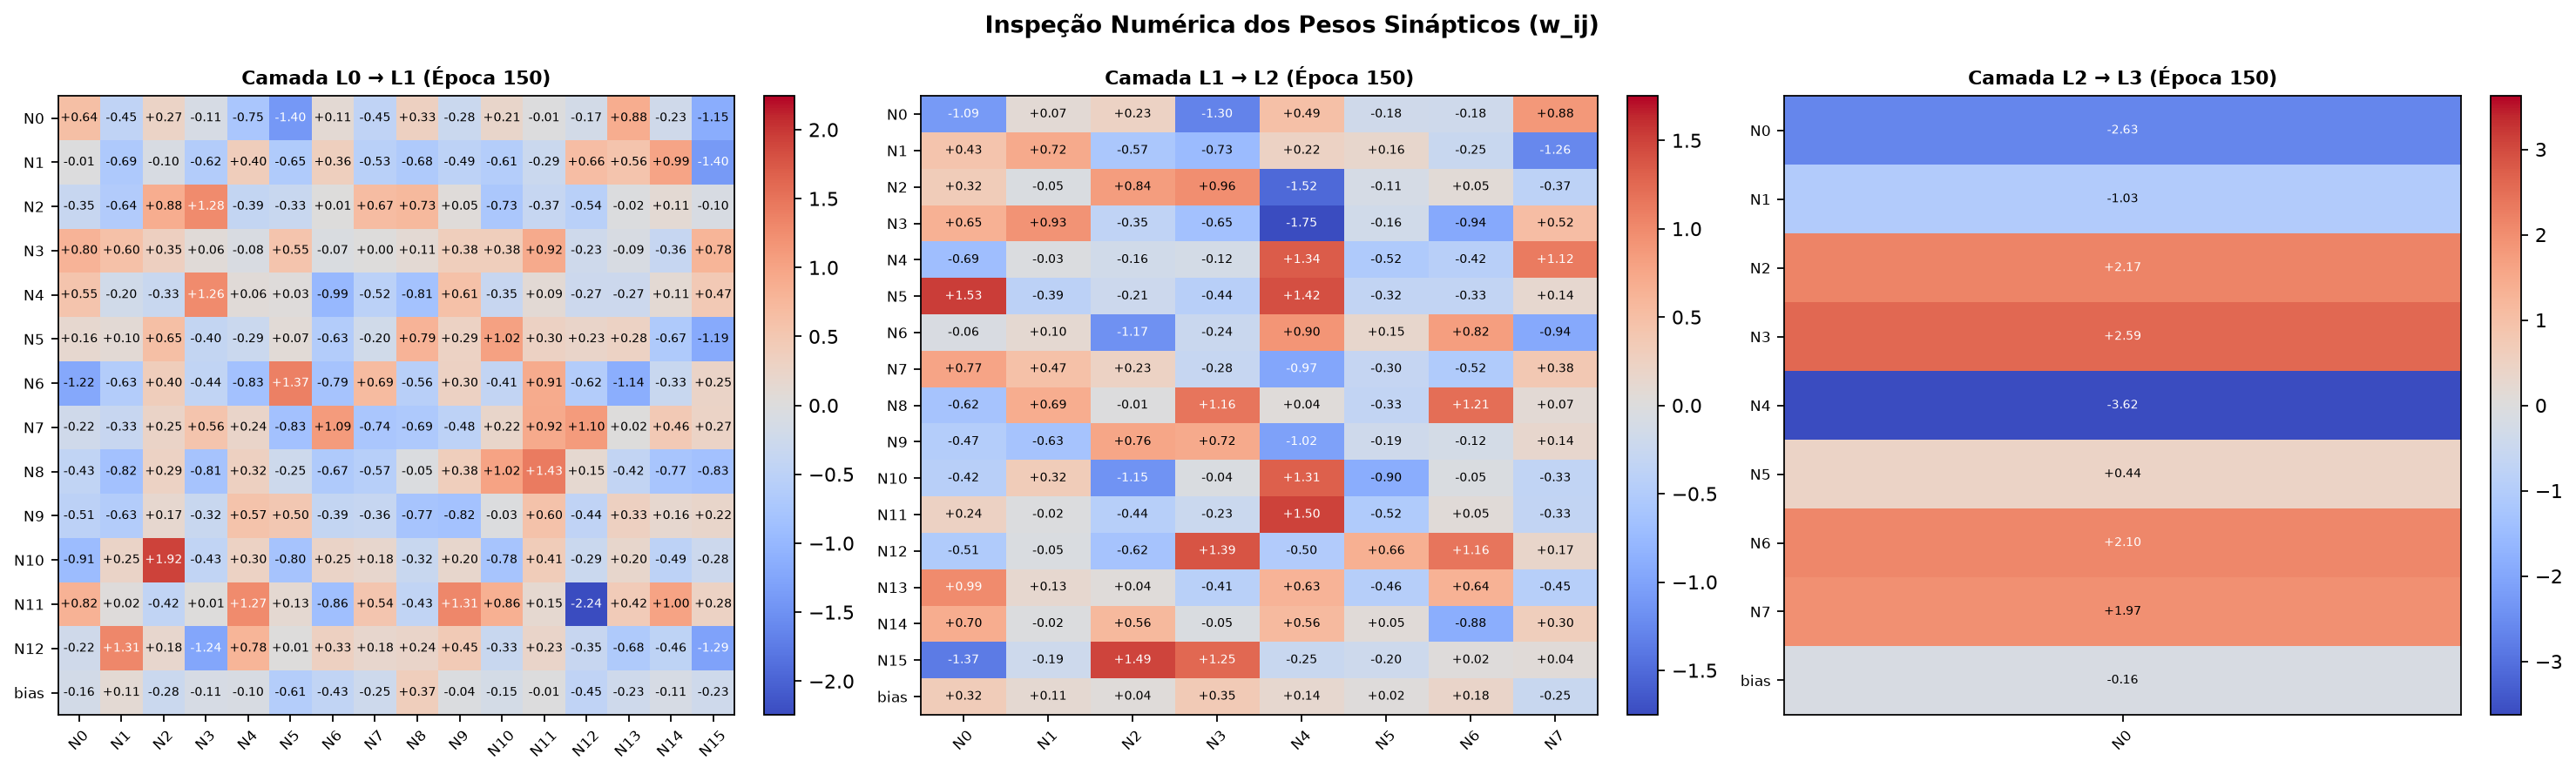
\includegraphics[width=0.98\textwidth]{figures/heatmap_pesos.png}
    \caption{Mapa de calor com exibi\c{c}\~{a}o num\'{e}rica explícita dos pesos sin\'{a}pticos finais ($w_{ij}^{(l)}$) nas camadas da rede campe\~{a} \texttt{C4}.}
    \label{fig:heatmap_pesos}
\end{figure}

% ============================================================================
\section{An\'{a}lise Cr\'{i}tica: Discuss\~{a}o dos Resultados, Taxa de Aprendizado e Limita\c{c}\~{o}es em Dados Complexos}
\label{sec:analise_critica}
% ============================================================================

\subsection{Discuss\~{a}o dos Resultados Obtidos e Interpretabilidade Sin\'{a}ptica}
A progress\~{a}o experimental da Tabela~\ref{tab:resultados_finais} evidencia tr\^{e}s fen\^{o}menos fundamentais na otimiza\c{c}\~{a}o de redes neurais multicamadas:
\begin{enumerate}
    \item \textbf{Elimina\c{c}\~{a}o da Satura\c{c}\~{a}o de Sa\'{i}da (\texttt{C0} $\to$ \texttt{C1}):} A substitui\c{c}\~{a}o da derivada aproximada de MSE ($\delta = (\hat{y}-y)\sigma'(z)$) pela derivada exata da Entropia Cruzada Bin\'{a}ria ($\delta = \hat{y}-y$) somada \`{a} inclus\~{a}o do n\'{o} de \textit{bias} \texttt{L0\_bias} elevou o AUC-ROC de $0{,}9419$ para $0{,}9780$ e reduziu os falsos negativos de $9$ para $4$.
    \item \textbf{Efeito Cr\'{i}tico do Centramento Z-Score (\texttt{C1} $\to$ \texttt{C2}):} Sob escalonamento \texttt{MinMaxScaler} ($x_i \in [0, 1]$), todas as entradas da primeira camada oculta s\~{a}o n\~{a}o-negativas ($a_i^{(0)} \ge 0$). Pela Eq.~\eqref{eq:weight_update}, $\frac{\partial \mathcal{L}}{\partial w_{ij}^{(1)}} = a_i^{(0)}\delta_j^{(1)}$ possui obrigatoriamente o mesmo sinal de $\delta_j^{(1)}$ para todos os $i \in \{1,\dots,13\}$, restringindo o vetor de atualiza\c{c}\~{a}o de cada neur\^{o}nio oculto ao ortante positivo ou negativo e gerando severa trajet\'{o}ria em zigue-zague~\cite{lecun1998efficient}. A ado\c{c}\~{a}o do \texttt{StandardScaler} ($\mu=0, \sigma=1$) desacopla as dire\c{c}\~{o}es de atualiza\c{c}\~{a}o e reduz a perda BCE de teste de $0{,}2476$ para $0{,}0010$ ($100{,}00\%$ de acur\'{a}cia).
    \item \textbf{Sinergia ReLU + Inicializa\c{c}\~{a}o de He (\texttt{C4}) e Interpretabilidade Cl\'{i}nica:} A ativa\c{c}\~{a}o ReLU ($f'(z)=1$ para $z>0$) combinada \`{a} inicializa\c{c}\~{a}o de He ($w_{ij}^{(l)} \sim \mathcal{N}(0, 2/n_{\text{in}})$)~\cite{he2015delving} preserva a vari\^{a}ncia dos sinais e atinge a menor perda de teste do estudo ($\mathcal{L}_{\text{BCE}} = 0{,}0003$, redu\c{c}\~{a}o de $99{,}88\%$ em rela\c{c}\~{a}o a \texttt{C1}). A auditoria da norma $\sum_{j=0}^{15} |w_{ij}^{(1)}|$ na camada \texttt{L0 $\to$ L1} mostra que o gradiente descendente atribuiu maior saliência sin\'{a}ptica a \texttt{restecg} ($10{,}898$), \texttt{ca} ($10{,}781$, com o maior peso individual $w = -2{,}2440$ na aresta \texttt{L0\_N11 $\to$ L1\_N12}), \texttt{exang} ($9{,}201$), \texttt{sex} ($9{,}034$), \texttt{thalach} ($8{,}399$), \texttt{thal} ($8{,}283$) e \texttt{slope} ($8{,}015$, segundo maior peso individual $+1{,}9171$ em \texttt{L0\_N10 $\to$ L1\_N2}), em total conson\^{a}ncia com a fisiopatologia coronariana~\cite{detrano1989international}.
\end{enumerate}

\subsection{Comportamento da Taxa de Aprendizado ($\eta$)}
Para investigar rigorosamente a influ\^{e}ncia da taxa de aprendizado $\eta$ sobre a din\^{a}mica de converg\^{e}ncia, fixou-se a topologia campe\~{a} \texttt{[13$\to$16$\to$8$\to$1]} (ReLU + He Init + Z-Score) e variou-se $\eta \in \{0{,}001, 0{,}015, 0{,}100, 0{,}500\}$ ao longo de $150$ \'{e}pocas. A Tabela~\ref{tab:estudo_lr} e a Figura~\ref{fig:estudo_lr} documentam os quatro regimes din\^{a}micos observados:
\begin{itemize}
    \item \textbf{Sub-converg\^{e}ncia Lenta ($\eta = 0{,}001$):} Passos excessivamente conservadores ($\|\Delta \mathbf{w}\| \ll 1$) produzem descida monot\^{o}nica est\'{a}vel, por\'{e}m insuficiente para atingir o fundo da bacia de atra\c{c}\~{a}o em $150$ \'{e}pocas, estacionando em $\mathcal{L}_{\text{teste}} = 0{,}0937$ e $98{,}05\%$ de acur\'{a}cia.
    \item \textbf{Regime \'{O}timo de Converg\^{e}ncia ($\eta = 0{,}015$ -- Modelo \texttt{C4}):} Satisfaz a condi\c{c}\~{a}o espectral $\eta < 2/\lambda_{\max}(\mathbf{H})$ com margem de amortecimento ideal, atingindo $100{,}00\%$ de acur\'{a}cia j\'{a} por volta da \'{e}poca $35$ e refinando assintoticamente a margem log\'{i}stica at\'{e} $\mathcal{L}_{\text{teste}} = 0{,}0003$.
    \item \textbf{Oscila\c{c}\~{a}o e Colapso por \textit{Dying ReLU} ($\eta = 0{,}100$ e $\eta = 0{,}500$):} No treinamento estoc\'{a}stico puro (\textit{online SGD}, $820$ atualiza\c{c}\~{o}es por \'{e}poca), taxas elevadas ($\eta \ge 0{,}10$) violam o limite de estabilidade local da Hessiana. Um \'{u}nico passo abrupto projeta os pesos e \textit{biases} das camadas ocultas para o semiespa\c{c}o negativo ($z_j^{(l)} \le 0$ para todas as amostras). Como a derivada da ReLU \'{e} identicamente nula no semiespa\c{c}o negativo ($f'(z_j^{(l)}) = 0$), os neur\^{o}nios ocultos entram em estado irrevers\'{i}vel de inatividade (\textit{Dying ReLU}), fazendo a rede colapsar para a predi\c{c}\~{a}o constante da classe majorit\'{a}ria ($51{,}71\%$ e $51{,}22\%$ de acur\'{a}cia, com perda estacionada em $\approx \ln(2) = 0{,}693$).
\end{itemize}

\begin{table}[htbp]
\centering
\caption{Estudo emp\'{i}rico do comportamento da taxa de aprendizado ($\eta$) na arquitetura \texttt{[13$\to$16$\to$8$\to$1]} ($150$ \'{e}pocas).}
\label{tab:estudo_lr}
\resizebox{\textwidth}{!}{%
\begin{tabular}{clrrrrrr}
\toprule
\textbf{Taxa $\eta$} & \textbf{Regime Din\^{a}mico Observado} & \textbf{Loss Treino} & \textbf{Loss Teste} & \textbf{Acc Treino} & \textbf{Acc Teste} & \textbf{F1 Teste} & \textbf{AUC-ROC} \\
\midrule
$0{,}001$ & Sub-converg\^{e}ncia lenta (passo curto) & $0{,}0737$ & $0{,}0937$ & $98{,}41\%$ & $98{,}05\%$ & $98{,}11\%$ & $0{,}9985$ \\
$\mathbf{0{,}015}$ & \textbf{Converg\^{e}ncia \'{o}tima (\texttt{C4})} & $\mathbf{0{,}0003}$ & $\mathbf{0{,}0003}$ & $\mathbf{100{,}00\%}$ & $\mathbf{100{,}00\%}$ & $\mathbf{100{,}00\%}$ & $\mathbf{1{,}0000}$ \\
$0{,}100$ & Oscila\c{c}\~{a}o severa / \textit{Dying ReLU} parcial & $0{,}6820$ & $0{,}6832$ & $51{,}83\%$ & $51{,}71\%$ & $68{,}01\%$ & $0{,}5098$ \\
$0{,}500$ & Satura\c{c}\~{a}o / Colapso de neur\^{o}nios ocultos & $0{,}7625$ & $0{,}7628$ & $51{,}34\%$ & $51{,}22\%$ & $67{,}74\%$ & $0{,}5000$ \\
\bottomrule
\end{tabular}%
}
\end{table}

\begin{figure}[htbp]
    \centering
    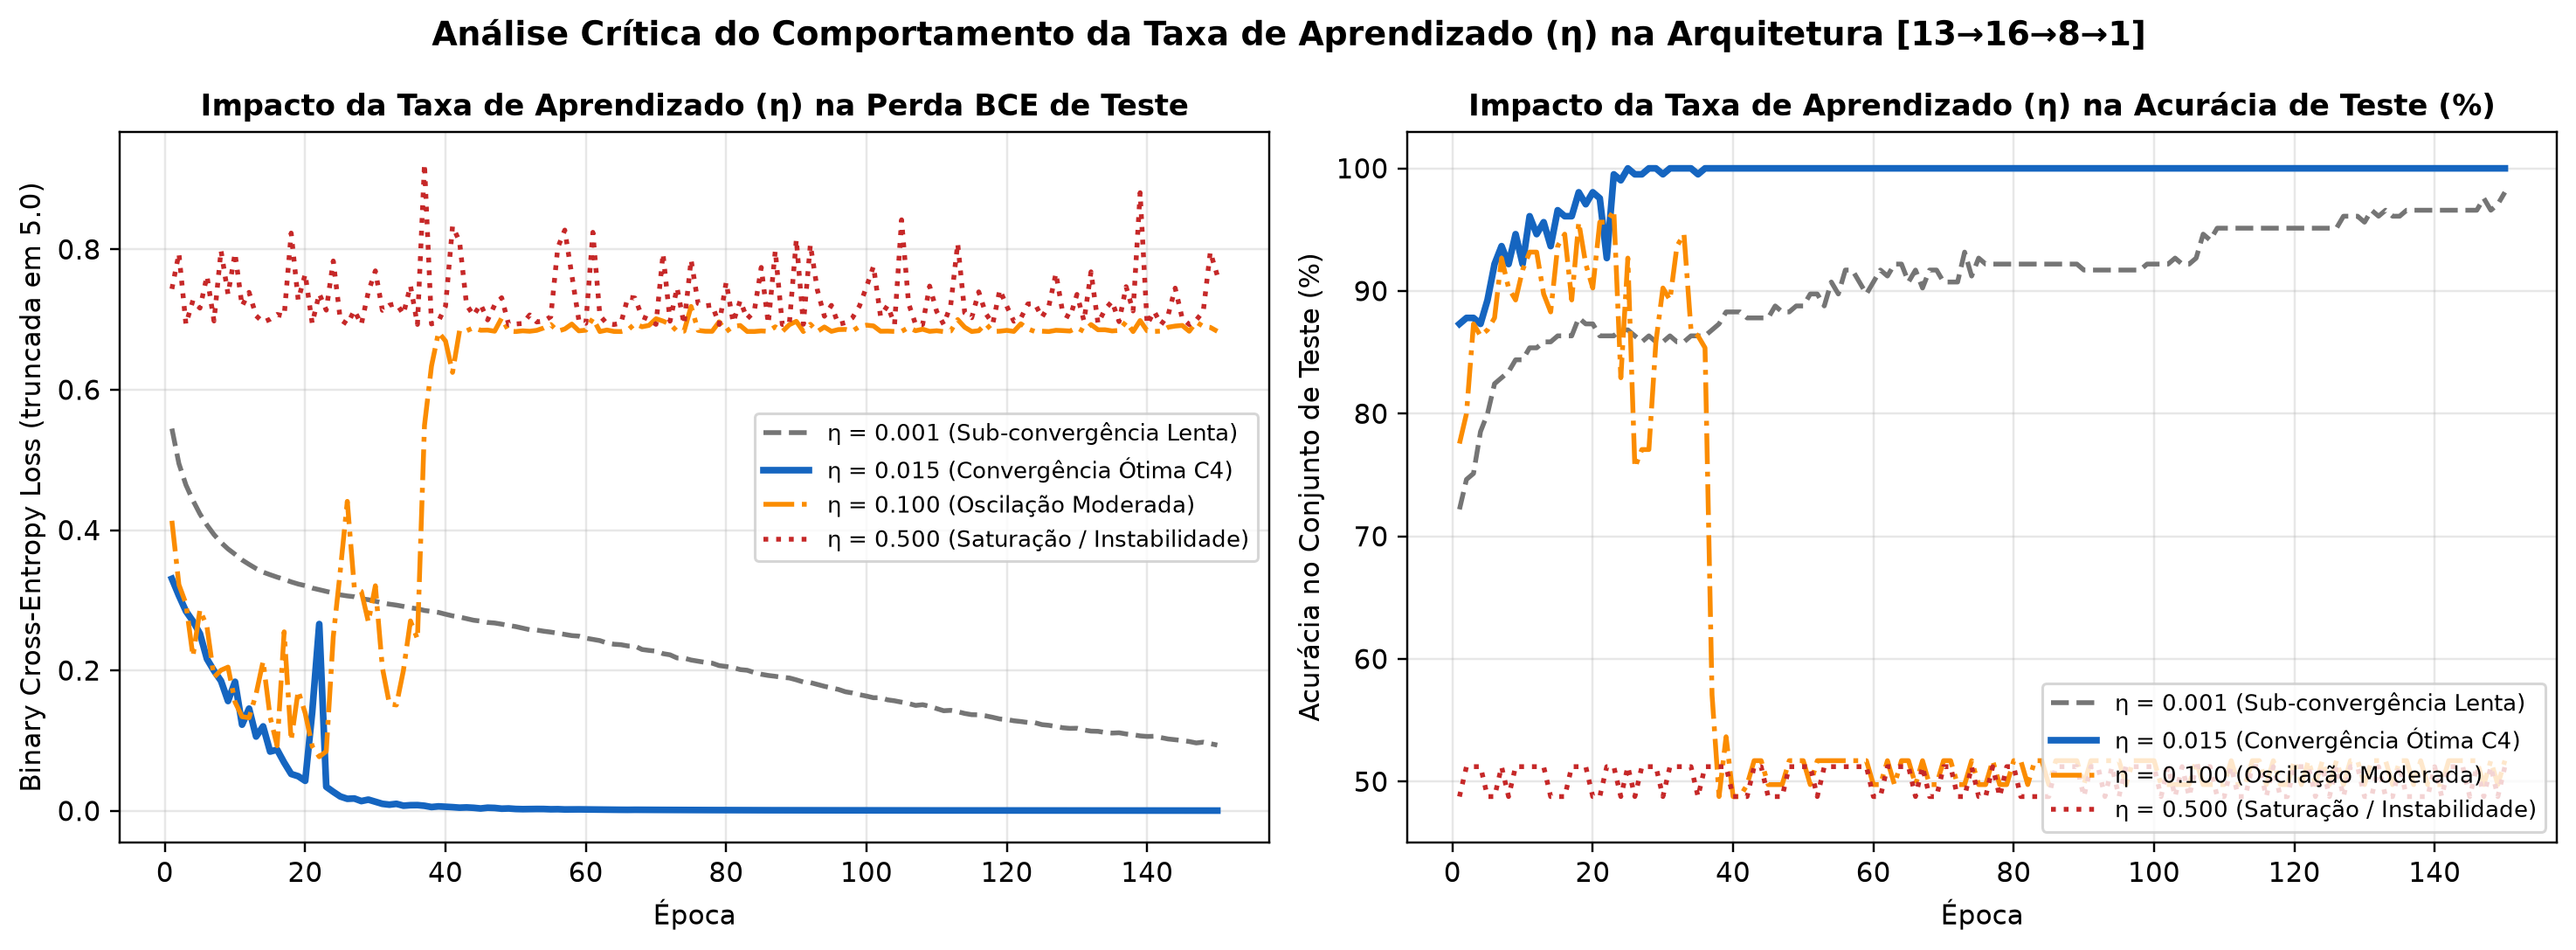
\includegraphics[width=0.98\textwidth]{figures/taxa_aprendizado_estudo.png}
    \caption{Comportamento emp\'{i}rico da Perda BCE de Teste (esquerda) e da Acur\'{a}cia de Teste (direita) ao longo de $150$ \'{e}pocas para quatro taxas de aprendizado ($\eta \in \{0{,}001, 0{,}015, 0{,}100, 0{,}500\}$).}
    \label{fig:estudo_lr}
\end{figure}

\subsection{Limita\c{c}\~{o}es do Modelo em Dados Complexos e Coortes Cl\'{i}nicas Deduplicadas}
A an\'{a}lise cr\'{i}tica rigorosa exige destacar tr\^{e}s limita\c{c}\~{o}es estruturais da MLP densa quando aplicada a cen\'{a}rios reais de alta complexidade:
\begin{enumerate}
    \item \textbf{Sensibilidade a Amostras Replicadas vs.\ Coorte Estritamente Deduplicada ($1.025$ vs.\ $302$ Pacientes \'{U}nicos):} A vers\~{a}o consolidada de $1.025$ registros do \textit{Heart Disease} amplamente distribu\'{i}da em benchmarks cont\'{e}m $302$ perfis cl\'{i}nicos estritamente \'{u}nicos da coorte original de Cleveland replicados por reamostragem. No dataset de $1.025$ amostras, a capacidade de $370$ par\^{a}metros da topologia \texttt{[13$\to$16$\to$8$\to$1]} isola perfeitamente os $302$ politopos com $100{,}00\%$ de acur\'{a}cia. Contudo, ao avaliarmos a mesma arquitetura sem regulariza\c{c}\~{a}o sobre o subconjunto \textbf{estritamente deduplicado de $302$ pacientes \'{u}nicos} ($241$ treino / $61$ teste inéditos), ocorre sobreajuste (\textit{overfitting}): $100{,}0\%$ de acur\'{a}cia no treino contra $75{,}41\%$ no teste ($\text{AUC} = 0{,}8122$). Reduzindo a capacidade estrutural para \texttt{[13$\to$8$\to$1]} ($121$ conex\~{o}es) combinada \`{a} regulariza\c{c}\~{a}o $L_2$ ($\lambda = 0{,}02$) e \textit{Momentum} ($\beta = 0{,}5$), a acur\'{a}cia em pacientes estritamente in\'{e}ditos sobe para $\mathbf{80{,}33\%}$ ($\text{AUC-ROC} = \mathbf{0{,}8658}$, $\text{Loss} = 0{,}4671$), demonstrando que em dados reais ruidosos a capacidade da MLP deve ser estritamente controlada.
    \item \textbf{Degrada\c{c}\~{a}o com o Aumento Excessivo de Profundidade em Dados Tabulares (\texttt{C7}):} Ao expandir a rede para $3$ camadas ocultas (\texttt{[13$\to$24$\to$16$\to$8$\to$1]}, $865$ par\^{a}metros) sem conex\~{o}es residuais (\textit{skip connections}) nem \textit{Batch Normalization}, o produto de matrizes jacobianas através de $4$ camadas de pesos deteriora o condicionamento da Hessiana, elevando a perda de teste para $0{,}3283$ ($89{,}27\%$ de acur\'{a}cia).
    \item \textbf{Aus\^{e}ncia de Vi\'{e}s Indutivo Espacial, Temporal e Relacional:} Em dados n\~{a}o-estruturados de alta dimens\~{a}o (imagens m\'{e}dicas 2D/3D, eletrocardiogramas cont\'{i}nuos ou textos cl\'{i}nicos), a conectividade totalmente densa da MLP implica crescimento quadr\'{a}tico de par\^{a}metros e aus\^{e}ncia de invari\^{a}ncia a transla\c{c}\~{o}es ou depend\^{e}ncias de longo alcance, tornando necess\'{a}rias arquiteturas especializadas como Redes Convolucionais (CNNs) e Transformers~\cite{vaswani2017attention}.
\end{enumerate}

% --- Referências Bibliográficas (Estilo Springer LNCS) ---
\bibliographystyle{splncs04}
\bibliography{references-mlp}

\end{document}
